\documentclass[12pt,twoside]{article}

% *** Set page dimensions ***
\raggedbottom
\parindent=0in
%\setlength{\topmargin}{-0.5in}
%\setlength{\oddsidemargin}{0.1875in}
%\setlength{\evensidemargin}{0in}
%\setlength{\textheight}{8.5in}
%\setlength{\textwidth}{6.225in}
%\addtolength{\oddsidemargin}{-0.7in}
%\addtolength{\evensidemargin}{-1.2in}
%\setlength{\oddsidemargin}{-0.2in}
%\setlength{\evensidemargin}{-0.2in}
%\addtolength{\textwidth}{1.4in}
%\addtolength{\topmargin}{-.875in}
%\addtolength{\textheight}{2.00in}

% *** Packages ***
\usepackage{alltt}
\usepackage{tocloft}
\usepackage{graphicx}
\usepackage{lscape}
\usepackage{amssymb}
\usepackage{float}
\usepackage{amsmath}
\usepackage{gensymb}
%\usepackage{subfigure}
\usepackage{lscape}
\usepackage{epsfig}
\usepackage{enumerate}
\usepackage{multicol}
\usepackage{fancyhdr}
\usepackage{epstopdf}
\usepackage{hyperref}
\usepackage{listings}

% *** Table of contents and Sectioning *** 
\setcounter{secnumdepth}{0}
\setcounter{tocdepth}{5}

% *** Table of contents and Sectioning *** 
\newcommand{\next}{\addtocounter{enumi}{9} \item}
\newcommand{\now}[1]{\setcounter{enumi}{#1}}
\newcommand{\Z}{\mbox{\sf Z\hspace{-1.5mm}Z}}
\newcommand{\R}{\mbox{\rm I\hspace{-0.75mm}R}}
\columnsep=0.75in

% *** Shortcuts for syntax ***
\newcommand{\ds}{\displaystyle }
\newcommand{\vsc}{\vspace{4mm}}
\newcommand{\dd}[1]{\frac{d}{d{#1}} \,} 
\newcommand{\ddx}{\frac{d}{dx} \,} 
\newcommand{\ddy}{\frac{d}{dy} \,} 
\newcommand{\ddz}{\frac{d}{dz} \,} 
\newcommand{\dydx}{\frac{dy}{dx} \,} 
\newcommand{\dydt}{\frac{dy}{dt} \,} 
\newcommand{\dfdx}{\frac{df}{dx} \,} 
\newcommand{\ddt}[1]{  \frac{d{#1}}{dt} }
\newcommand{\pp}[2]{  \frac{\partial{#1}}{\partial {#2}} }
\newcommand{\zx}{\frac{\partial z}{\partial x} \,}
\newcommand{\zy}{\frac{\partial z}{\partial y} \,}
\newcommand{\limh}{\lim_{h \rightarrow 0} \;}
\newcommand{\diff}{\frac{d}{dx} \,}
\newcommand{\de}{\Delta}
\renewcommand{\thesection}{\Roman{section}}
\newcommand{\bfr}{\begin{flushright}}
\newcommand{\efr}{\end{flushright}}
\newcommand{\dx}{\frac{\partial f}{\partial x} \,}
\newcommand{\dy}{\frac{\partial f}{\partial y} \,}
\newcommand{\p}{\partial}
\newcommand{\vi}{\vec{i}}
\newcommand{\vj}{\vec{j}}
\newcommand{\vk}{\vec{k}}
\newcommand{\lan}{\left\langle}
\newcommand{\ran}{\right\rangle}
\newcommand{\reading}[1] { {\em Reading: #1}}
\renewcommand{\Pr}{ \mbox{Pr}}

% *** Commands related to textbook references
\newcommand{\problem}{{\bf Problem.} }

% *** Footnoting with symbols ***
\long\def\symbolfootnote[#1]#2{\begingroup%
\def\thefootnote{\fnsymbol{footnote}}\footnote[#1]{#2}\endgroup}

% *** Defining a boxed note ***
\floatstyle{boxed}
\newfloat{noteinbox}{htb}{loa}
\newenvironment{boxnote}{\begin{noteinbox}[H]}{\end{noteinbox}}

\newcommand{\Question}{ {\bf Question: }  }
\newcommand{\Example}[1]{ {\bf Example: } {\em #1} }
\newcommand{\ExampleCont}[1]{ {\em #1} }

% *** Define the boxed Week #/summary at the beginning/end of every chapter ***
\newcommand{\sectionbox}[1]{% 
\begin{tabular}{|p{6in}|}%
\hline%
\ \\ %
{\Large {\bf {#1}}}  \\%
\ \\%
\hline%
\end{tabular}}

% *** Shortcuts *** 
\newcommand\goals{\large {\bf {Goals:}}}
\newcommand\setfont{ }

% *** Week commands: overwritten in each notes file
\newcommand{\Week}{Null-InPreambleCommon}
\newcommand{\WeekTitle}{Null-InPreambleCommon}
\newcommand{\Course}{MNTC P04}
\newcommand{\SetNum}{1 }
\newcommand{\topic}[1]{
\newpage
\setcounter{page}{1}
\fancyhead[LE,RO]{#1 - \thepage}
}

% *** Setup Latex for the large version of the files ***
%\usepackage[landscape]{geometry}
\usepackage[letterpaper,landscape,hmargin={.8in,.8in},vmargin={1in,0.2in}]{geometry}

% Remove paragraph indents
\setlength{\parindent}{0pt}

% Spacing at the top for the header is too large by default
\setlength{\voffset}{-5ex}

% **** RENEW SCALING COMMANDS HERE ****
% *** Text in boxes ***
\renewenvironment{boxnote}{\begin{noteinbox}[H] \huge}{\end{noteinbox}} 

% *** Chapter lead in/summary boxes ***
\renewcommand{\sectionbox}[1]{% 
\begin{tabular}{|p{9.5in}|}%
\hline%
\ \\ %
{\huge {\bf {#1}}}  \\%
\ \\%
\hline%
\end{tabular}}

% *** 'Section'' commands, which are sometimes used for spacing
% From http://zoonek.free.fr/LaTeX/LaTeX_samples_section/0.html
\makeatletter
 \renewcommand\section{\@startsection {section}{1}{\z@}%
                                    {-3.5ex \@plus -1ex \@minus -.2ex}%
                                    {0.3ex \@plus.2ex}%
                                    {\setfont\bf}}

 \renewcommand\subsection{\@startsection {subsection}{1}{\z@}%
                                    {-3.5ex \@plus -1ex \@minus -.2ex}%
                                    {0.3ex \@plus.2ex}%
                                    {\setfont\bf}}

% *** 'Goals' should be larger in the overheads ***
\renewcommand\goals{\huge {\bf {Goals:}}}
\renewcommand\setfont{\huge }

\thispagestyle{empty}

\setfont 

\newcommand{\WeekTitleOne}{Derivatives - Foundations}
\newcommand{\WeekTitleTwo}{Derivatives - Linearization and Applications}
\newcommand{\WeekTitleThree}{Derivatives - Modeling}
\newcommand{\WeekTitleFour}{Integrals - Foundations}
\newcommand{\WeekTitleFive}{Integrals - Techniques}
\newcommand{\WeekTitleSix}{Integrals - Modeling}
\newcommand{\WeekTitleSeven}{Differential Equations - }
\newcommand{\WeekTitleEight}{Differential Equations - }
\newcommand{\WeekTitleNine}{Differential Equations - }
\newcommand{\WeekTitleTen}{Linear Algebra - }
\newcommand{\WeekTitleEleven}{Linear Algebra - }
\newcommand{\WeekTitleTwelve}{Linear Algebra - }



\begin{document}
\setfont
\pagestyle{fancy}
\renewcommand{\Week}{3 }
\renewcommand{\WeekTitle}{\WeekTitleThree }

\fancyhead[LE,RO]{Week \Week}  % default, usually only for first page
\fancyfoot{}
\sectionbox{Week \#\Week: \WeekTitle}


\vspace{5mm}
\goals
\begin{itemize}
\item Calculate and interpret the first and second derivatives, as
  well as higher order derivatives.
\item Define and calculate Taylor polynomials.
\item Use MATLAB to graph and compare functions with their Taylor
  polynomial approximations.
\item Find and use critical points for global and local optimization
  problems.
\item Use MATLAB optimizers and equation solvers to identify optimal
  values and critical points.
\end{itemize}

\vspace{5mm}


\newpage
\topic{Second and Higher Derivatives}
\subsection*{Second and Higher Derivatives}


A lot of information about the graph of a function $f$ can be deduced
by the sign of $f'(x)$ and $f''(x)$ (the {\bf second derivative} of
$f(x)$) on an interval $(a,b)$.

{\huge
\vsc
\begin{center}
\begin{tabular}{|l|l|} \hline
\qquad \qquad \qquad \qquad \qquad  \qquad \qquad & \qquad  \qquad \qquad \qquad \qquad  \qquad \qquad \\
\qquad $f'(x) > 0 {\mbox{ on }} (a,b)$  &  \qquad $f$ increasing on $[a,b]$  \\
\qquad \qquad \qquad \qquad \qquad & \qquad \qquad \qquad  \qquad \qquad \\
 \hline
\qquad \qquad \qquad \qquad \qquad & \qquad \qquad \qquad  \qquad \qquad \\
\qquad $f'(x) < 0 {\mbox{ on }} (a,b)$  &  \qquad $f$ decreasing on $[a,b]$  \\
\qquad \qquad \qquad \qquad \qquad & \qquad \qquad \qquad  \qquad \qquad \\
 \hline
\qquad \qquad \qquad \qquad \qquad & \qquad \qquad \qquad  \qquad \qquad \\
\qquad $f''(x) > 0 {\mbox{ on }} (a,b)$  &  \qquad $f$ concave up on $[a,b]$  \\ \qquad \qquad \qquad \qquad \qquad & \qquad \qquad \qquad  \qquad \qquad \\
\hline
\qquad \qquad \qquad \qquad \qquad & \qquad \qquad \qquad  \qquad \qquad \\
\qquad $f''(x) < 0 {\mbox{ on }} (a,b)$  &  \qquad $f$ concave down on $[a,b]$ \qquad  \qquad  \\ 
\qquad \qquad \qquad \qquad \qquad & \qquad \qquad \qquad  \qquad \qquad \\
\hline
\end{tabular}
\end{center}
}
\setfont

\newpage 

\problem Sketch the possible graphs combining different signs of
positive and negative first and second derivatives.

\vfill
\vfill


\problem Sketch graphs where the {\bf first} derivative has a zero value. 

\vfill \problem Sketch graphs where the {\bf second} derivative has a
zero value.

\vfill

\newpage

Aside from their graphical interpretation, the second derivative
frequently has an important physical meaning in kinematics problems.

\problem If $x(t) = 4 \sin(2t)$ gives the position of a particle at
time $t$, what is particle's {\bf speed} at $\ds t=\frac{\pi}{6}$?

\vfill

For the same particle, what is its {\bf acceleration} at
$\ds t=\frac{\pi}{6}$?

\vfill

\newpage



While their interpretations are not as immediately obvious, it is also
possible to compute 3rd, 4th, or higher derivatives of function if we
want.

\problem Find the first four derivatives of the function
$$f(x) = 7 e^{-2x} + \ln(x).$$


\newpage
\topic{Taylor Polynomials}
\subsection*{Taylor Polynomials}

One application of higher derivative information is to help us build
{\bf polynomial approximations} to other functions.

Previously we found a formula for linear approximations to functions
$f(x)$ around a point $x=a$:

\vspace{1.5in}

This linear approximation, or tangent line formula, can also be called
the {\bf Taylor polynomial of degree 1 approximating $f(x)$ near
  $x=a$.}

\newpage

\problem Sketch the graph of $\cos(x)$ around $x=0$, and add its
tangent line based at $x=0$.


\includegraphics[width=3in]{graphics/empty_graph_square_12}


The linearization or tangent line is clearly a very
  limited approximation to this function.  What might be a {\em
    slightly} more complex form of function that would work better in
  this case?

\vfill

\newpage

\begin{boxnote}

{\bf Taylor Polynomial of Degree 2}
\vspace{1in}

$$ f(x) \approx ~~~~~f(a) ~~~~~+ f'(a) (x-a) ~~~~~+ \frac{f''(a)}{2} (x-a)^2$$  

\vspace{1in}

is a {\em quadratic} approximation to $f(x)$ near $x=a$.
\end{boxnote}


\problem For values of $x$ close to $a$ do you think this quadratic
approximation will be a better or worse approximation than the tangent
line?  Why?

\vfill

\newpage

\problem Find the quadratic Taylor approximation to \\$f(x) = \cos(x)$
  near $x=0$.

\vfill

\newpage

\problem Use MATLAB to draw the graph of $\cos(x)$ around $x=0$, and
add both its 1st and 2nd degree Taylor polynomial approximations for
$x$ near 0.


\newpage
$$ f(x) \approx f(a) + f'(a) (x-a) + \frac{f''(a)}{2} (x-a)^2$$  

The form of the coefficients in the Taylor polynomial are carefully
chosen.

\problem What mathematical features will the original $f(x)$ share
with its 2nd degree Taylor approximation at the point $x=a$?

\vfill

\newpage
\topic{Taylor Polynomials of Higher Degree}
\subsection{Taylor Polynomials of Higher Degree}

\problem If we wanted a still-better approximation for a function
$f(x)$ near a specific point $x=a$, how could we generalize our
earlier 1st and 2nd degree Taylor polynomials?

\vfill

\newpage 

Below is the general formula for the terms in a Taylor polynomial, up
to degree $n$.  \\
\begin{boxnote} ~\\[1ex]
$$ f(x) \approx ~~f(a) ~~+ f'(a) (x-a) ~~+ \frac{f''(a)}{2} (x-a)^2 + \ldots 
+ \frac{f^{(n)}(a)}{n!} (x-a)^n$$    \\[-0.5ex]
\end{boxnote}
\begin{itemize}
\item $f^{(n)}$ means ``the $n$-th derivative of $f$''. \\
\item $n!$ means ``$n$ factorial''
\end{itemize}

\newpage
\subsection*{Higher Degree Taylor Polynomials - Example 1}

Consider the function $f(x) = \sin(x)$.

\problem Find the first five derivatives of $f(x)$, and evaluate them at $x=0$.


\newpage

\problem Write out the Taylor polynomial of degree 5 for
$f(x) = \sin(x)$.

\vfill

\problem Write out the general form of the Taylor polynomial of degree
$n$ for $f(x) = \sin(x)$.

\vfill

\newpage

\problem Use MATLAB to plot the graph of $f(x) = \sin(x)$ and the
Taylor polynomial approximations up to degree 5.

\newpage

MATLAB Demo of even higher degree Taylor approximations to $\sin(x)$.

\newpage


\topic{Higher Degree Taylor Polynomials - Example 2}
\subsection*{Higher Degree Taylor Polynomials - Example 2}

Consider the function $g(x) = x e^{-x}$.

\problem Find the first three derivatives of $g(x)$, and evaluate them
at $x=1$.


\newpage

\problem Write out the Taylor polynomial of degree 3 for \\
$g(x) = x e^{-x}$ centered at $x=1$.

\vfill

\newpage

\problem Use MATLAB to plot the graph of $g(x) = x e^{-x}$ and the
Taylor polynomial approximation from degree 1, 2 and 3.

\newpage
\topic{Critical Points}

\subsection*{Critical Points} 

Aside from understanding the shape of functions, derivative
information can help us identify and classify interesting points of a
function, like the highest and lowest values.

\problem Sketch graphs which have high and low points.  

\vfill 

What do those extreme values have in common?


\newpage

To help identify local extreme values, we introduce the definition of
a critical point.

\begin{boxnote}

  If $f(x)$ is defined on the interval $(a,b)$, then we call a point
  $c$ in the interval a {\bf critical point} if:
\begin{itemize}
	\item $f'(c) = 0$, or
	\item $f'(c)$ does not exist.
\end{itemize}
We will also refer to the point $(c,f(c))$ on the graph of $f(x)$ as a
critical point.  We call the function value $f(c)$ at a critical point
$c$ a {\bf critical value}.

\vsc
\end{boxnote}

\newpage

Technical Notes:
\begin{enumerate} 
\item By this definition, $f(c)$ must be {\bf defined} for
  $c$ to be a critical point.  

\problem   Sketch $f(x) = 1/x$, and decide whether $x=0$ is a
    critical point.

\vfill
  Sketch $g(x) = |x|$, and decide whether $x=0$ is a
    critical point.

\vfill

\newpage

\item By the definition, if a function is defined on a closed
  interval, the endpoints of interval {\bf cannot} be critical points.

\problem   Sketch the graph of $f(x) = \sqrt{x}$ and decide
    whether $x=0$ is a critical point.

\vfill

\newpage

\problem Sketch the graph of $g(x) = \sqrt[3]{x}$ and decide
  whether $x=0$ is a critical point.

\vfill

\end{enumerate}

\newpage

% \problem Identify all the critical points on the graph below, and
%   characterize any other interesting points by continuity, limits, or
%   other properties.

\problem Identify all the critical points on the graph below.

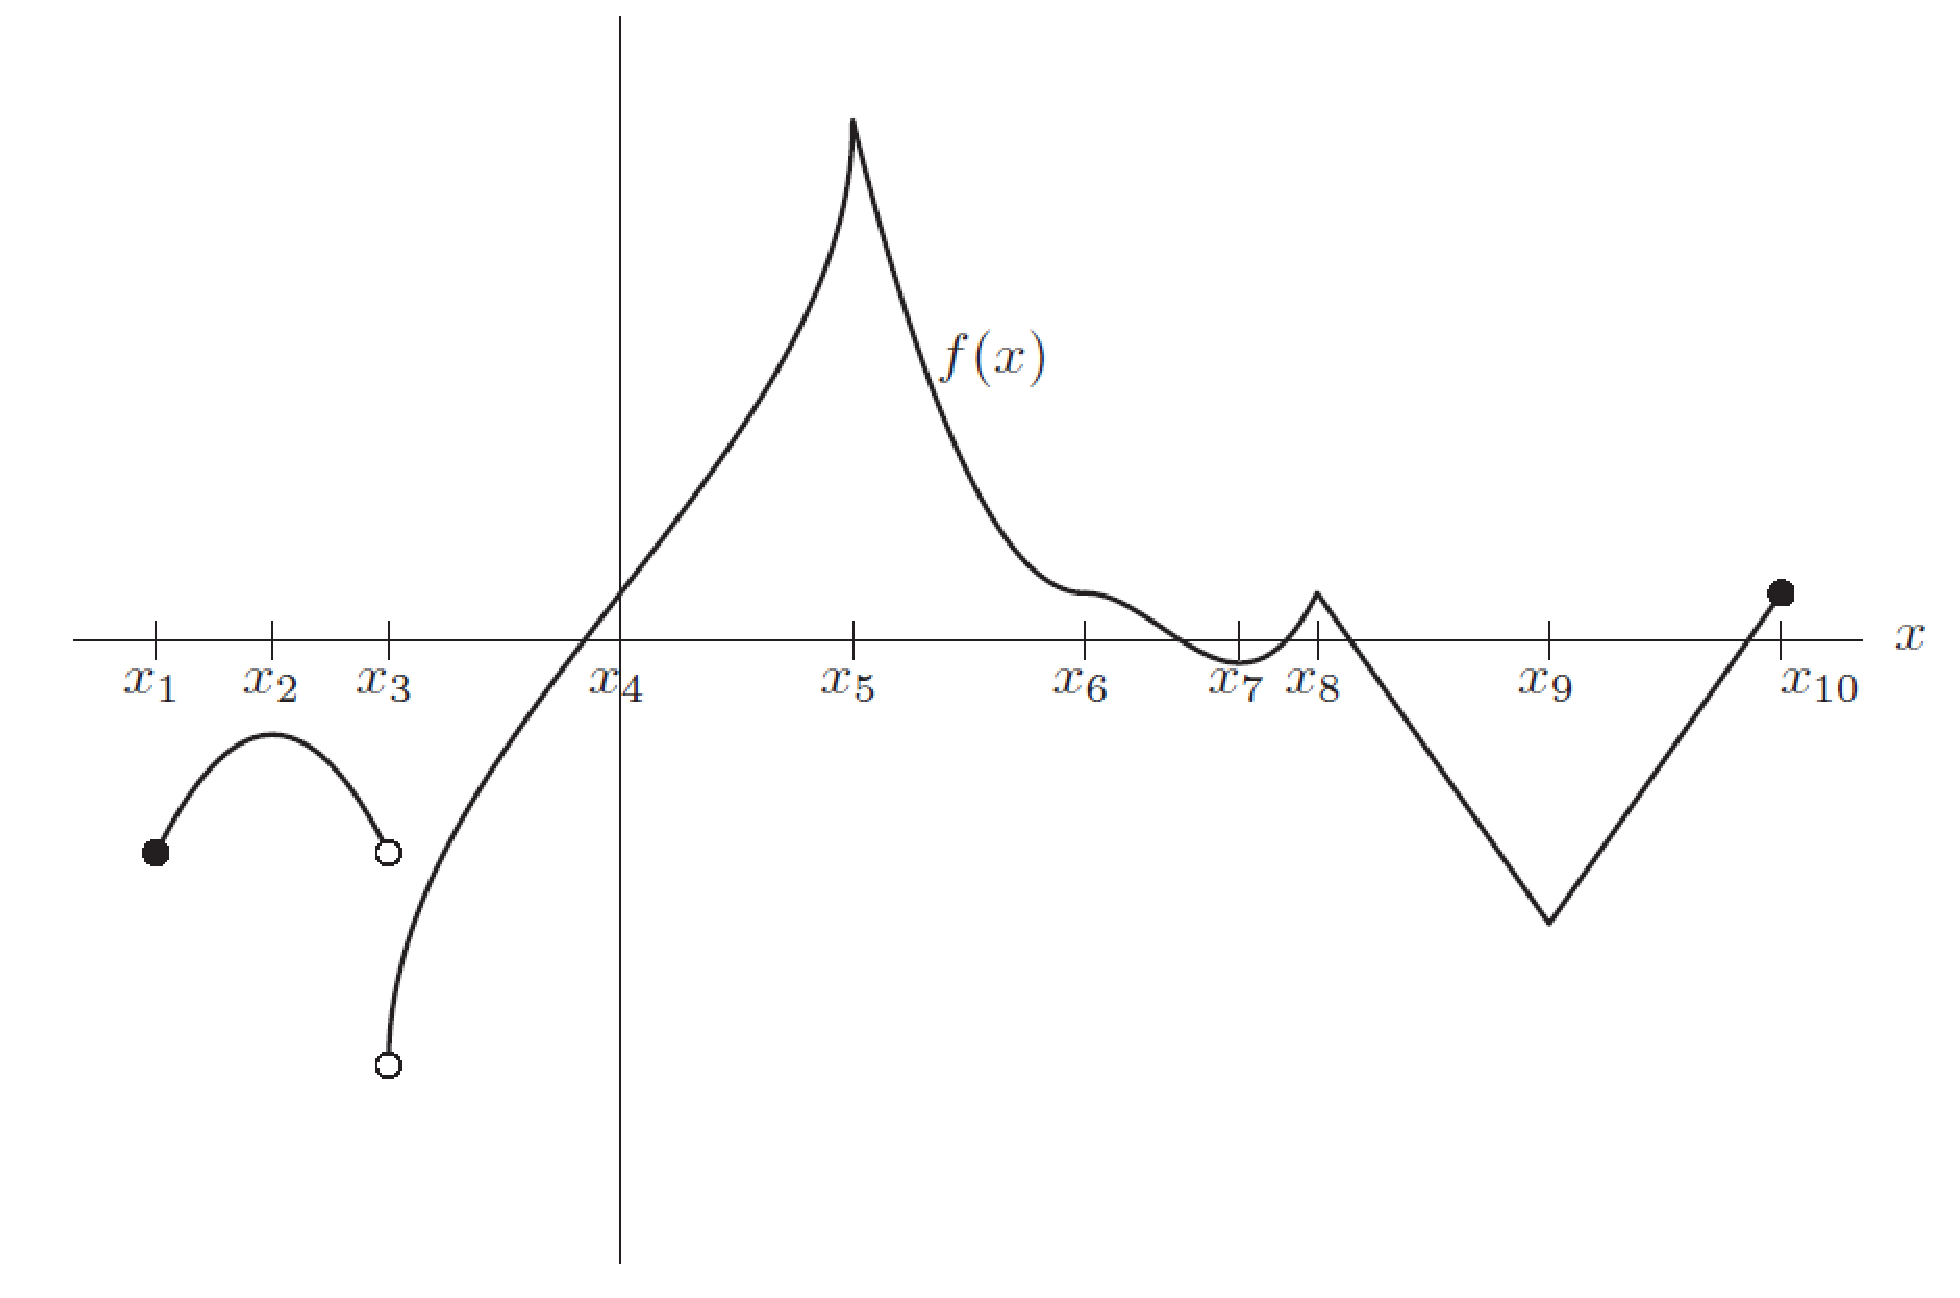
\includegraphics[width=8in]{graphics/notes_03_crit_pnt_oddities}

\newpage

\topic{Classifying Critical Points}

\section*{Classifying Critical Points}

We will now formalize two ways to determine if a critical point is a
local min, max, or neither. This avoids the need for a sketch of the
graph. \\[2ex]
\newpage
{\bf First Derivative Test}

One indicator of the type of critical points is the sign of the
derivative on each side of the critical point.  This classification
method is called the {\bf{first derivative test}}.

\problem Complete this table:
{\LARGE
\vspace{1mm}
\begin{center}
\begin{tabular}{|l|c|c|p{2.1in}|} \hline
\qquad \qquad \qquad \qquad \qquad &  $f'$ sign left of $c$ & $f'$ sign right of $c$ & Sketch of $f(x)$  \\ \hline
local minimum at $c$ & & &\\[1.0in] \hline
local maximum at $c$ & & &\\[1.0in] \hline
neither local max nor min & & &\\[1.0in] \hline
\end{tabular}
\end{center}
}

%\def\arraystretch{1}
\vspace{1.5mm}


\newpage

\problem Find the critical points of the function
$$f(x) = 2 x^3 - 9 x^2 + 12 x +3.$$ Use the first derivative test to
show whether each critical point is a local maximum or a local
minimum.

\vfill
\vfill

\newpage 

\problem Using your answer to the preceding question, determine the
number of real solutions of the equation
$2 x^3 - 9 x^2 + 12 x + 3 = 0$.

\vfill

\newpage 
\begin{boxnote}
{\bf Second Derivative Test}

You may also use the Second Derivative Test to determine if a critical
point is a local minimum or maximum.  
\begin{itemize}
\item The first derivative test uses the {\bf first} derivative {\bf
    around} the critical point.
\item The second derivative test uses the {\bf second} derivative {\bf at} the critical point.
\end{itemize}
\begin{itemize}
\item If $f'(c)$ = 0 and $f''(c) > 0$ then $f$ has a local minimum at $c$. \\[2ex]
\item If $f'(c)$ = 0 and $f''(c) < 0$ then $f$ has a local maximum at $c$. \\[2ex]
\item If $f'(c)$ = 0 and $f''(c) = 0$ then the test is inconclusive. \\[2ex]
\end{itemize}
\end{boxnote}

\vsc
\newpage
\problem A function $f$ has derivative $f'(x) = \cos(x^2) + 2x - 1$.
  Does it have a local maximum, a local minimum, or neither at its
  critical point $x=0$?

\newpage 

\topic{Global vs. Local Optimization}
\section*{Global vs. Local Optimization}

The first and second derivative tests only give us {\em local}
information in most cases.  However, if there are multiple local
maxima or minima, we usually want the {\bf global} max or min.  The
ease of determining when we have found the global max or min of a
function depends strongly on the properties of the question.

\begin{boxnote}

  \subsection*{Local vs Global Extrema}

  A {\bf local max} occurs at $x=c$ when $f(c) > f(x)$ for $x$ values
  near $c$.

  A {\bf global max} occurs at $x=c$ if $f(c) \ge f(x)$ for {\bf all}
  values of $x$ in the domain.  

  It is possible to have several global maxima if the function reaches
  its peak value at more than one point.

  Corresponding definitions apply for local and global minima.

\end{boxnote}

\newpage

\problem Give an example of a simple function with multiple global
  maxima.

\vfill

\problem Give an example of a simple function with a single global
  maximum, but no global minimum.

\vfill

\problem Give an example of a simple function with neither a global
  maximum nor a global minimum.

\vfill


\newpage Earlier we worked with the function $$f(x) = 2 x^3 -
  9 x^2 + 12 x +3.$$  
\problem If we limit the function to the interval $x \in
  [0, 2.5]$, what are the {\bf global max} and {\bf global minimum}
  values on that interval?  



\vfill
\vfill

Confirm your answer using MATLAB to plot the graph of $f(x)$.

\newpage

\topic{Global Extrema on Closed and Open Intervals}

\begin{boxnote}
\subsection*{Global Extrema on Closed Intervals}

A continuous function on a closed interval will {\bf always} have a
global max and a global min value.  These values will occur at either
\begin{itemize}
\item a critical point {\em or}
\item an end point of the interval.
\end{itemize}
To find which value is the global extrema, you can compute the
original function's values at all the critical points and end points,
and select the point with the highest/lowest value of the function.

\end{boxnote}


\newpage
\begin{boxnote}
\subsection*{Global Extrema on Open Intervals}

A function defined on an open interval may or may not have global
maxima or minima.  
\vsc

If you are trying to demonstrate that a point is a global max or min,
and you are working with an open interval, including the possible
interval $(-\infty, \infty)$, proving that a particular point is a global
max or min requires a careful argument.  A recommendation is to look
at either:
\begin{itemize}
\item values of $f$ when $x$ approaches the endpoints of the interval,
  or $\pm \infty$, as appropriate; or
\item if there is only one critical point, look at the sign of $f'$ on
  either side of the critical point.
\end{itemize}
With that information, you can often construct an argument about a
particular point being a global max or min.

\end{boxnote}

\newpage

\problem Determine whether the function
$$f(x) = 2 x^3 - 9 x^2 + 12 x +3$$ has a global max and/or min.

\vfill


\newpage
\problem Determine whether the function $f(x) = (x-2)^4$ has a global
  max and/or min.

\vfill

\newpage

\topic{Optimization - Fencing Example}
\section*{Optimization}

An optimization problem is one in which we have to find the maximum or
minimum value of some quantity.  In principle, we already know how to
find the maximum and minimum values of a function if we are given a
formula for the function and the interval on which the maximum or
minimum is sought.  Usually the hard part in an optimization problem
is interpreting the word problem in order to find the formula of the
function to be optimized.

\vsc 

\newpage 

\problem A site manager wants to build a rectangular security fence to
surround a site.  The manager has 480 meters of wire fencing with
which to build a fence, and one side of the enclosure will be part of
the side an already existing building (so there is no need to put up
fence on that side). What should the dimensions of each side be to
maximize the area enclosed?

\vsc


What is the quantity to be maximized in this example?

\vspace{2cm}

\newpage

\problem What are the variables in this question, and how are they
related?  You may want to draw a picture.

\vfill

Express the quantity to be optimized in terms of the
  variables.  Try to eliminate all but one of the variables.

  \vfill

  What is the domain on which the one remaining variable
    makes sense?

\vspace{2cm} 
  \newpage 

  \problem Use the techniques learned earlier in the course to
  maximize the enclosed by the fence.  Give reasons explaining why the
  answer you found is the {\bf global} maximum.

\vspace{5cm}

\newpage

\hfill (continued)

\vfill

\problem Confirm your solution using a MATLAB graph of your function
for the enclosed area.  \vspace{1in}



\newpage

\topic{Optimization - Storage Example}
\problem (Storage Container)\\ A rectangular storage container with an
  open top is to have a volume of 10 m$^3$.  The length of its base is
  to be twice its width.  Material for the base costs \$10.00 per
  m$^2$, and material for the sides costs \$6.00 per m$^2$.  Determine
  the cost of the material for the cheapest such container.

~ \hfill 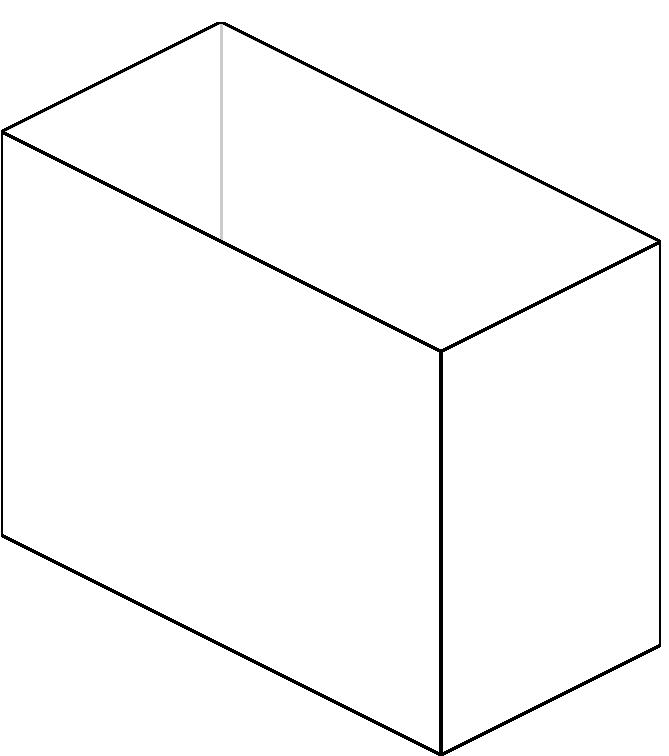
\includegraphics[width=1.5in]{graphics/notes_03_storage_container}

\newpage
~ \hfill 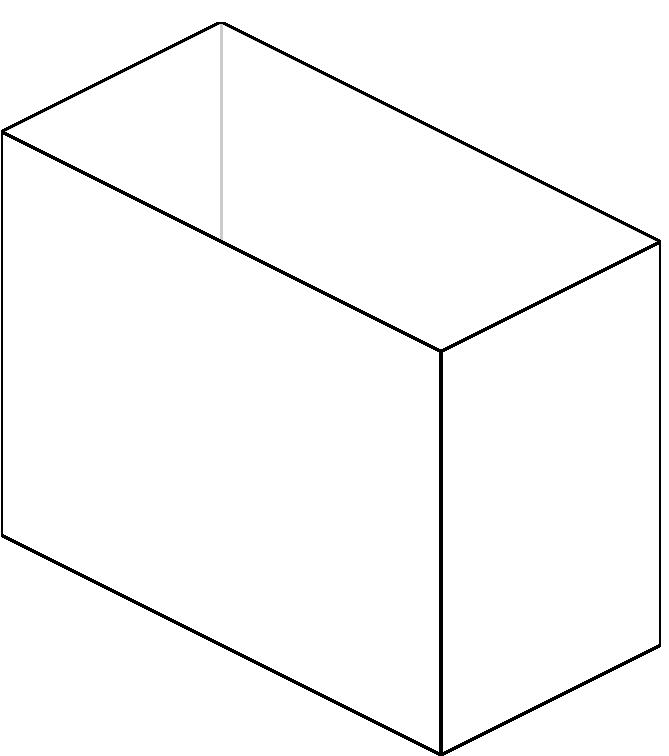
\includegraphics[width=1.5in]{graphics/notes_03_storage_container}

\newpage
~ \hfill 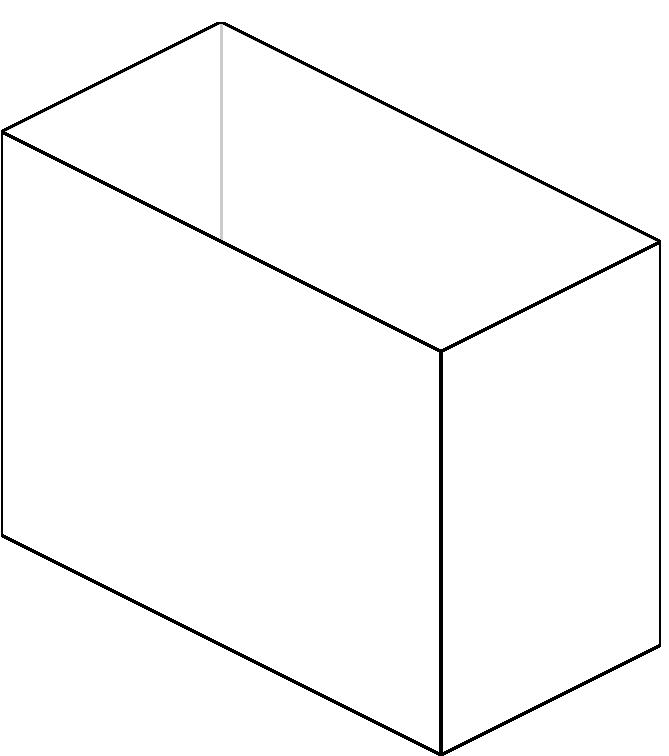
\includegraphics[width=1.5in]{graphics/notes_03_storage_container}

\newpage

\topic{Optimization in MATLAB}
\subsection*{Optimization in MATLAB}

MATLAB has built-in numerical methods tools that can also perform
optimization, given the formula for a function.  However, those tools
have the same limitations as our earlier work with numerical methods
for solving equations.

These {\bf numerical methods} are all {\bf fancy versions of guess and
  check}!  This means numerical solutions are a poor second choice,
compared to by-hand solving:
\begin{itemize}
\item Numerical optimums give no insight into the optimal value
  (existence, patterns).
\item Finding numerical optimums usually requires some amount of trial
  and error by the user.
\end{itemize}

Despite these limitations though, numerical methods are great in that
they can be applied to any function, and don't require any by-hand
solving for critical points.

\newpage

{\bf Defining New MATLAB Functions}

User-written functions are an important tool in MATLAB.  For purposes
of our optimization problems, we will use the simplest implementation,
called {\bf anonymous functions}.

\begin{verbatim}
f = @(x)  x.^2;

x = linspace(-2, 2);
plot(x, f(x)); 
\end{verbatim}

\newpage

{\bf Optimizing MATLAB functions} 

The single-variable optimization function in MATLAB is called \texttt{fminbnd}.

\problem Look at the help menu for \texttt{fminbnd}. 
\vfill


\newpage

\problem Use \texttt{fminbnd} to find a minimum of
$f(x) = e^{-x} + x$.

\vfill

Graph $f(x) = e^{-x} + x$ and add a point at the minimum that was
found.
\vfill

\newpage
\problem Use \texttt{fminbnd} to find the global minimum of \\
$g(x) = x \sin(x)$ on the interval $x \in [0, 4\pi]$.

\vfill

Graph $g(x)$ and comment on steps you need to take to find the global
minimum.
\vfill

\newpage

\topic{MATLAB Optimization - Further Examples}
\subsection*{MATLAB Optimization - Further Examples}

You'll notice that command \texttt{fminbnd} does {\bf not} have a
sister function \texttt{fmaxbnd}.  Instead, MATLAB requires users to
turn any maximization problem they have into a minimization problem
themselves. \\[1ex]
 
\begin{minipage}[t]{0.6\linewidth}
  
\problem Sketch a graph $y = f(x)$ which has a local maximum.
\vspace{2in}

Now sketch the graph of $y = -f(x)$.  

What do you notice about the $x$ locations of the minima on this
function?  
\vspace{1in}~
\end{minipage}


\newpage
\problem Use \texttt{fminbnd} to find the global {\bf maximum} of \\
$g(x) = x \sin(x)$ on the interval $x \in [0, 4\pi]$.

\newpage
\problem Use \texttt{fminbnd} to find the length of side fence $x$
that maximizes an enclosed rectangular area, if one side is against
the wall.  The total length of fence is 480 m.

$\displaystyle A(x) = x \frac{(480-x)}{2}$

\vfill

Also find the total area enclosed with the optimal design.  \vspace{1in}

\newpage
\problem Use \texttt{fminbnd} to find the length of the box sides that
minimizes the cost of building an open-topped storage container whose
materials cost \$10 per m$^2$ for the base, and \$6 per m$^2$ for the
sides.  The box must have a final volume of 10 m$^3$.

$\displaystyle C(x) = 10 x^2 + (6) (4 x \left(\frac{10}{x^2}\right))$
\vfill

Also find the total cost of the optimal design.  \vspace{1in}




\newpage

{\bf Notation Confusion}

There is an unfortunate coincidence in MATLAB notation that often
catches new users.

\problem Contrast the meaning of the \texttt{y(1.5)} in these two
MATLAB examples.


\begin{minipage}[t]{0.45\linewidth}
\vspace{0pt}
\begin{verbatim}
x = linspace(-2, 2);
y = x.^2;

y(1.5)
\end{verbatim}
\end{minipage} \hfill
\begin{minipage}[t]{0.45\linewidth}
\vspace{0pt}
\begin{verbatim}
x = linspace(-2, 2);
y = @(x)  x.^2;

y(1.5)
\end{verbatim}
  
\end{minipage} 





\end{document}

